\documentclass[conference]{IEEEtran}
\IEEEoverridecommandlockouts
% The preceding line is only needed to identify funding in the first footnote. If that is unneeded, please comment it out.
\usepackage{cite}
\usepackage{amsmath,amssymb,amsfonts}
\usepackage{algorithmic}
\usepackage{graphicx}
\usepackage{textcomp}
\usepackage{xcolor}
\usepackage{xspace}
\def\BibTeX{{\rm B\kern-.05em{\sc i\kern-.025em b}\kern-.08em
    T\kern-.1667em\lower.7ex\hbox{E}\kern-.125emX}}


\DeclareEmphSequence{\bfseries}
\def\projname{ImageInThat\xspace}

%ImageInThat: Manipulating Image and Language to Convey Intent to Robots

\newcommand{\mk}[1]{\textcolor{cyan}{[todo: #1]}}

\newcommand{\figref}[1]{Fig. \ref{#1}}

\def\virtualized{\textsc{virtualized}\xspace}

\definecolor{lightgrey}{rgb}{0.8,0.8,0.8}
\definecolor{white}{rgb}{1.0,1.0,1.0}

\newcommand{\highlighted}[2]{\emph{#1} #2}

% remove after diffing
% \usepackage{tikz}
% \DeclareRobustCommand\circled[2]{\tikz[baseline=(char.base)]{
%             \node[shape=circle,draw,inner sep=0, minimum size=1em,preaction={fill, #1}] (char) {\textbf{#2}};}}
% \newcommand{\highlight}[2]{\emph{#1} \circled{lightgrey}{#2}}
    
\begin{document}

\title{\projname: Manipulating Image and Language \\ to Convey User Intent to Robots}

\maketitle

\begin{abstract}
    Robots are becoming increasingly capable of responding to humans' natural language instructions to perform everyday manipulation tasks such as wiping a table or meal preparation. However, natural language presents challenges, such as ambiguity in spatial instructions (e.g., choosing a specific apple from a basket) and requiring users to mentally track how the robot’s state evolves during long-horizon tasks. In this work, we propose using images as an alternative paradigm to instruct robots. We introduce \projname, a specific instantiation of this paradigm, which allows users to perform direct manipulation on images in a timeline-style interface to generate step-by-step robot instructions. Through a user study with twelve participants we evaluated \projname for instructing robots on kitchen manipulation tasks, comparing it to a text-based timeline. The results show that \projname was faster, led to fewer errors, and was preferred by participants over the text-based interface. We also demonstrate that image-based instructions can be translated into robot executable policies, and discuss the potential of combining the strengths of language and images to create multimodal robot instructions.

    % Robots are becoming increasingly capable of performing everyday tasks through modern foundation models, yet end-users still need to provide input to surface preferences and constraints to enable successful completion of tasks in their environments. Natural language is often considered an effective means for this two-way communication. However, it can be challenging for robots to communicate their actions in a way that is quickly understood and contextualized within the environment. Conversely, users may struggle to instruct the robot on changes to its task plans due to language ambiguities and the complexities of managing language over long-duration tasks. We propose a novel system, PhotoManipulator, which uses generated images to describe the robot’s task plans to the end-user. Through direct manipulation and interaction with the images of the task plans, PhotoManipulator surfaces user preferences and constraints that can be reused in future task iterations. Through user studies with X participants, we demonstrate that programs were easier to create and edit using PhotoManipulator when compared to a language-only interface.
\end{abstract}

\begin{IEEEkeywords}
component, formatting, style, styling, insert
\end{IEEEkeywords}

\section{Introduction}
\bla{Another random thought, but I think we should pick an application domain like household tasks and make it clear we are not stepping outside of that.}

\bla{I think this paragraph justifies the need for user intervention versus a fully autonomous ``interaction'', but I think it should instead spend one sentence justifying that, and more sentences justifying why more methods for creating and interpreting instructions for robots are needed. I.e. issues with representing instructions with language, or end user programming. I also think the reasons for needing user intervention are multifaceted, and more than just generic models don't adapt to user preferences. I think there's other issues such as models not actually performing well enough, and I think there's likely a user desire for more control over the model https://dl.acm.org/doi/abs/10.1145/3290605.3300750

I'd also maybe love a simpler, more straighforward and attention grabbing hook here.

``Advances in foundation models are improving the capabilities of autonomous robots at the pace of leaps and bounds instead of baby steps; we find ourselves on the cusp of having robots in our homes, in a world where we no longer have to do the dishes. (maybe some examples from the literature). However, the need for human instruction of robots is still needed. Whether it is limitations of the models, strict and unknown human preferences, a desire from humans for controllability, or simply the entry point for a human to instruct a robot, even once foundation models are in our homes, we will still need to instruct them.''}


%\mk{Computers \dots}
%The advancement of large foundation models that process combination of language and vision has made robots more intelligent and capable of performing complex tasks.
Robots are becoming increasingly autonomous and capable of performing complex tasks through the advent of robot foundation models. Thus, we expect that robots will aid us in completing everyday tasks in the near-term. While these models are trained on internet-scale data, they do not understand the specific environment they will operate in. Thus, they will still need to attend to instructions from users~\cite{ajaykumar2021survey}. Imagine a user asks a robot to put away newly purchased groceries in the kitchen. The robot, following a generic organisation procedure, might randomly store canned goods and cereals together based on the space available inside. However, the user might organize their cabinet in a more nuanced way, such as by placing heavier items on lower shelves due to their cabinet's fragility and lighter items above for easier lifting. They might also want daily-use items such as cereal in the front, even if it blocks other items. As a result, the user would need to intervene and adjust the robot’s approach to match their environment and preferences.

\bla{If our goal is to position images in the landscape of techniques for instructing robots, I think we should stray away from comparing to language so much and instead make a general claim that the underlying problem we are solving are *many* drawbacks across different methods of instructing. For instance, interpreting end user programs is very difficult, language is difficult because of ambiguity, teleop requires an immense amount of concentration and has primarily been explored for real-time tasks not future tasks. The time spent manipulating for teleop is 1-1, so why wouldn't you do household tasks yourself.}

As it is expected that most users of future robots will not be experts, natural language has been touted as a modality that people can use to instruct robots~\cite{tellex2020robots}. From a technical standpoint, state-of-the-art robot policies often utilize language-conditioning to generate robot actions. Despite the ubiquity of language and its easy-to-use interface, language is not always ideal. Natural language can be abstract and difficult to ground in the physical context. For instance, \textit{``Put the cereal in the cabinet'' }is unclear if there are many boxes of cereal and several cabinets to put them away inside of. Hence, the user needs to be more precise to achieve the desired result: \textit{``Put the blue cereal box into the top left corner of the middle cabinet next to the other cereal''}, or alternatively, provide corrections to a simpler instruction by uttering language~\cite{zha2023distilling}. Beyond the immediate problem of specifying instructions, the user faces the additional challenge of predicting how the robot's planned actions will affect the environment, particularly for long-horizon tasks.

\bla{Again, too much focus on language if we are positioning the paper in the overall landscape of robot instruction techniques. ``In this paper we propose the idea of directly manipulating images of the environment as a means of  instructing a robot. Compared to existing methods, images are easy to interpret, and because of their concrete grounding in reality do not suffer from issues with ambiguity.'' the last sentence needs work. The key thing is pulling language out of the topic sentence, and instead focusing on addressing drawbacks of other instruction methods in the literature.

Overall I like this paragraph a lot though. Teasing out some of these axes along which images differ from other techniques will be super important.}

Instead of solely using natural language as a means for instructing robots, we propose the use of images---both as a means for providing instructions to a robot, and for the robot to communicate what its plans are to the user. Images provide two main benefits over language. First, images are inherently easier to ground, as they visually represent the environment from which they originate. Hence, users should be able to contextualize the robot's current and future states through images. Second, by forming an appropriate representation of the environment as an image, we can enable direct manipulation~\cite{shneiderman1983direct}, which could be faster than forming precise language to resolve ambiguity and provide clear instructions. In addition, by supporting direct manipulation, the robot can develop a representation of the user's intent informed by their actions, and use this to intelligently propose future appropriate actions.

\bla{This is great I love this section. I'd love some more details on features of the system here though, we can make room for it in the intro by tightening the paragraphs above.}

We introduce a specific instantiation of this paradigm, \projname, where users can manipulate images of the environment to create instructions for a robot. In a user study with twelve participants, we compared \projname to a language-based method for several instruction following tasks in simulated kitchen environments. We found that participants were able to generate instructions in these tasks faster and with less errors when using \projname, and participants were more confident that their instructions could be understood by a robot when directly manipulating images that our prototype supports. We also demonstrate that instructions created using \projname can be used to perform robot manipulation tasks on a physical robot arm setup. Lastly, we discuss how the two modalities of language and image can be used in a complementary fashion to create \textit{multimodal instructions}.


% Recently, researchers have explored different techniques to allow end users to provide clarifications and corrections to robots that plan using large language models (a class of FMs). In these systems, step-by-step procedures are represented as natural language, and the end user can provide feedback on the robot's procedure or actions through language~\cite{zha2023distilling, mahadevan2024generative}. 
% % Challenge

% % Hook
% Something about LLMs/VLMs/robotics that we now have access to intelligent robotic models. Now we can do NLP-based programming of robots!

% % Challenge
% Language on its own is insufficient and can have issues. Plus models these days are vision-based (not sure if we need to include this)

% % Contribution
% We propose a novel interface that treats image as a first-class citizen. Image for input/output/errors

% % Evaluation
% We evaluated BLAH BLAH using BLAH BLAH.


\section{Related Work}
There exists a spectrum of robotic systems, ranging from those designed to create reusable, repeatable routines (i.e., using end-user robot programming~\cite{lieberman2006end, ajaykumar2021survey}) to those enabling real-time control (i.e., teleoperation). Our system falls somewhere in between, blending elements of both approaches.

\emph{End-user robot programming.} Prior work can be largely categorized into natural language-based and visual-based methods. Many systems employ speech for programming~\cite{cakmak2014teaching, gorostiza2011end}, though challenges remain in recognition and creating complex programs through continuous dialogue. Other approaches use text-based programming with visual scaffolds like blocks~\cite{huang2017code3, huang2016design, weintrop2018evaluating} or nodes~\cite{alexandrova2015roboflow,porfirio2018authoring}. Recently, large language models (LLMs) have been employed for text-based interactions, often via chat interfaces~\cite{karli2024alchemist, ge2024cocobo}. However, language input demands precision, especially for spatial tasks in robotics~\cite{masson2024directgpt, sundaresan2024rt}. Other systems span a range of visual modalities, such as augmented reality~\cite{ikeda2024programar, suzuki2022augmented, quintero2018robot, gong2019projection, cao2019ghostar}, spatial interfaces~\cite{huang2020vipo, cao2019v, mahadevan2022mimic}, sketch-based systems~\cite{sakamoto2009sketch, porfirio2023sketching}, physical demonstrations~\cite{akgun2012trajectories}, and tangible interaction~\cite{sefidgar2017situated, gao2019pati}. Despite the richness of prior EURP systems, they often require adherence to specific system rules. For instance, AR-based trigger-action programming~\cite{ikeda2024programar} necessitates precise trigger and action specifications within the user's AR environment. Moreover, many prior systems use intermediate representations (e.g., flow diagrams or blocks) to convey user intent. In contrast, \projname enables users to directly manipulate images to represent a desired world state without an intermediate representation.

% Mention ~\cite{li2022scene} at some point.

% FrameKit: A Tool for Authoring Adaptive User Interfaces Using
% Keyframes

% Montage: A Video Prototyping System to Reduce
% Re-Shooting and Increase Re-Usability

% Gaze+Hold: Eyes-only Direct Manipulation with Continuous
% Gaze Modulated by Closure of One Eye

% Authoring Sensor-based Interactions by Demonstration
% with Direct Manipulation and Pattern Recognition

% Multimodal Direct Manipulation in Video Conferencing:
% Challenges and Opportunities

% Representation
% Blocks: Code3 ~\autoref{huang2017code3, huang2016design, weintrop2018evaluating}
% Natural language: Alchemist ~\autoref{karli2024alchemist, ge2024cocobo}
% Spatio-visual: ~\autoref{huang2020vipo, senft2021situated}
% Demonstration + visual: ~\autoref{mahadevan2022mimic, porfirio2019bodystorming}

%% Augmented reality: ~\autoref{ikeda2024programar, suzuki2022augmented, quintero2018robot, gong2019projection, cao2019ghostar}
%% Tangible: ~\autoref{sefidgar2017situated, gao2019pati}
%% Sketch: ~\autoref{porfirio2023sketching, sakamoto2009sketch}

% Things to mention
% - the type of representations thaat people use like block/tangible/etc.
% - types of logic that programming has supported: loops/conditionals/
% - granularity of program: low vs high level

%https://dl.acm.org/doi/pdf/10.1145/2909824.3020249

% \cite{huang2022inner} also explores the idea of using feedback but the feedback can come from several sources like automated success detectors, scene descriptors like object detection modules, and human feedback. Precursor to works like distillation but still valid and relevant.

%\cite{yao2022react} A generalist paper that is talking about how LLMs on the whole can use language feedback to modify task-level step-by-step plans

% \cite{yu2023language} Also talks about using language but to generate rewards for robot skills. Similar to mine but uses a module to generate rewards and a motion controller instead of APIs.

% \cite{kwon2023toward} Use VLM and LLM loops to reason about things in a visual manner. In this manner, it is sort of suggesting that we don't necessarily need humans as much, but still a point towards visual information matters. Probably can borrow their motivation portions. In fact, they answer the question about commonsense but state clearly that somethings (and they have proof with user studies) are subjective like dirtiness. They even show that this improves overall grounded reasoning.

% \cite{hunt2024survey} Read and include if necessary.

% \subsection{End-User Robot Programming}
% %Can model after 2.2 of https://arxiv.org/pdf/2406.00841.
% End-user robot programming (EURP) aims to allow non-coders to program robot behaviors~\cite{lieberman2006end,ajaykumar2021survey}.
% Early EURP tools tapped into showing users graphical representations of robot programs, such as flow diagrams~\cite{alexandrova2015roboflow,porfirio2018authoring}.
% As these methods still require users to have some levels of understanding about a robot's available low-level actions, other work looked into programming robots by directly demonstrating desired behaviors through kinethestic teaching~\cite{akgun2012trajectories} or teleoperation~\cite{kitagawa2023online}.
% Another line of work explored using visual mark-ups on environments to set robot trajectories and points of interests~\cite{cao2019v,liu2011roboshop}.  
% However, these methods could not directly capture people's high-level goals, requiring them to sometimes arduously specifying individual actions.
% One exception is RT-Sketch~\cite{sundaresan2024rt}, which could interpret high-level state change goals from users' sketches of desired world states.
% However, as these sketches only captured object contours, they are limited in expressing object articulation and distinguishing similar objects.

% Recent advances in AI has enabled users to program high-level robot behaviors through natural language~\cite{tellex2011understanding,liang2023code,winge2024talk}.
% While expressive, natural language commands come with ambiguity that makes programming often more effortful than expected~\cite{stegner2024understanding}.
% Some recent work combined visual editing with natural language input to resolve ambiguity and simplify verbal expressions~\cite{porfirio2023sketching}.
% This research builds on existing work that leverages the complementary strengths of language and visual editing, and expands the expressiveness of visual editing by introducing object manipulation and state change generation.

% \subsection{Human-in-the-Loop Robot Planning}
% With the advent of robot foundation models, end-users may not need to program their robots completely from scratch as many prior systems assume. Instead, the end user's role may be to steer the model to plan towards their desired goals. Prior work has explored human-in-the-loop planning approaches to correct robots acting autonomously. In these settings, language has been seen as a natural fit to express user corrections or clarifications. For instance, it has been used to provide iterative corrections~\cite{zha2023distilling} that the robot can distill knowledge from in a future task (e.g., how to set a table) or to accelerate learning from specific users~\cite{liang2024learning}. It has been used to generate reward functions~\cite{yu2023language} or code~\cite{mahadevan2022mimic} to generate social robot behaviors. \projname enables user manipulations on images to refine and correct robot plans.

\emph{Live Robot Control} 
Modern robotic systems often include interfaces for the real-time teleoperation of the robots' joint and end-effector positions.
These interfaces are often based on graphical user interfaces (GUIs) or joysticks, offering immediate feedback for the controllers to adjust their input~\cite{darvish2023teleoperation,rea2022still}.
While effective, GUI- and joystick-based control mechanisms are cognitively and physically taxing for human operators, as they demands mental rotation and managing multiple separate degrees of freedom (DoFs) simultaneously.
To alleviate this burden, one thread of recent teleoperation research aims to directly map human motion to robot motion, often from the motion of human hands to robot end-effectors~\cite{rakita2017motion,rakita2019shared,fu2024mobile}.
Other work opts for a shared-control approach, where some trajectory prior informs a robot to generate high DoF trajectories from low DoF input.
Such prior is often derived from inferred operator goals~\cite{huang2016anticipatory,jain2019probabilistic,losey2022learning}.
Despite the assistance available, live control methods still require operators' continuous mental and physical engagement to manage robots' low-level motion.
Therefore, PhotoManipulator, along with other recent research, seeks to enable robots to interpret and execute human operators' high level intents.


\emph{Helping robots follow human instructions.} With the advent of foundation models (FM), end-users may not need to program their robots from scratch (as with EURP). Recent work has successfully deployed pre-trained LLMs for robotics tasks such as translating language instructions to policy code~\cite{liang2023code, singh2023progprompt, liu2024ok, mahadevan2024generative}. Previous work has demonstrated that language can be used to iteratively guide and correct robots, enabling them to learn from these interactions and apply that knowledge in future tasks~\cite{zha2023distilling, liang2024learning}. In contrast, other work has attempted to translate human instructions into robot actions directly by training robotic foundation models (RFM~\cite{kawaharazuka2024real}). Some of these techniques can generate actions when provided natural language inputs~\cite{driess2023palm, kim2024openvla}, such as, ``Bring me the chips from the drawer''. Alternatively, images can be used to represent goals, either as sub-steps of a task~\cite{black2023zero, nair2020contextual} or the final desired state~\cite{team2024octo, kapelyukh2023dall}. There are also attempts at using other modalities, including representing goals as sketches~\cite{sundaresan2024rt}, or desired trajectories overlaid on images~\cite{gu2023rt}. Our framework realized through \projname, is agnostic to the method used to provide instructions to the robot. This flexibility is achieved by separating the user's input representation when providing instructions from the representation used by the execute the instructions. For example, images can be captioned and sent as language instructions to a language-conditioned RFM. Alternatively, pre-trained models can translate images into executable code using existing skill primitives (e.g., picking up a coffee mug). The images can also be directly provided to an image-conditioned RFM.

%Prior work has shown that image-conditioned policies currently outperform language-conditioned policies~\cite{team2024octo} possibly as images inherently contain more concrete information about how to perform a task in a given environment. Our work, \projname, is partially motivated by the need to create images to serve as an input for goal-conditioned robot policies.

%To our knowledge, prior work (with the exception of RT-Sketch~\cite{sundaresan2024rt}) has assumed that goals can be autonomously generated (e.g., as in \cite{black2023zero}) to handle users' language instructions. This can be problematic both due to artifacts (an inherent limitation of diffusion models) and difficulties in precisely translating language instructions into images representing the user's desired goals. In contrast, we introduce \projname as a method to enable users to directly create images that represent sub-steps that a robot should execute using image-conditioned robot policies.

%\cite{winge2024talk} Kind of relevant with the idea of end user adaptation of an existing robotic system but really not that interesting.

%\cite{stegner2024understanding} Generalist paper about on-the-fly EURP. Might be able to refer to some of the challenges when talking about our solution (though we aren't fully building an EURP but it is the building blocks towards it to an extent).
%e.g. Theme 1: End users viewed program steps to better understand the system: Relevant because we allow this
%e.g. heme 4: End users had mixed experiences on interaction with the program synthesizer: Want to ensure our system provides users a sense of being in control
%\mk{Talk about EURP work that uses image editing/sketch/environment editing.}
%\cite{liu2011roboshop,skubic2007using} sketch-based interface for mobile robot control (little manipulation).
%\cite{sundaresan2024rt} allows users to draw object contours to specify desired environmental changes. 


%\cite{} Survey on EURP so regardless of anything we'd need to cite it.

% \subsection{Interfaces for Authoring and Browsing Spatial Content}
% Our prototype of \projname is directly inspired by significant HCI research into developing direct manipulation interfaces as well as interaction techniques for editing using keyframes.

% \emph{Direct manipulation.} Prior work in HCI has explored the use of direct manipulation, an interaction style where objects of the interface can be interacted with via physical, reversible, and incremental actions and that provide immediate feedback~\cite{shneiderman1982future, shneiderman1983direct}. For instance, videos can be scrubbed by directly manipulating the content rather than the timeline~\cite{dragicevic2008video, karrer2008dragon}. Direct manipulation has also been used to support the navigation of 3D spatial recordings~\cite{lilija2020put, xia2018spacetime}. It has been used to support drawing tools to visualize data~\cite{xia2018dataink, kim2019datatoon}, make procedural art~\cite{jacobs2017supporting}, programming SVGs~\cite{hempel2016semi}, and creating illustrations~\cite{xia2016object}. Direct manipulation has seen some application in robotics, including for programming robot swarms~\cite{suzuki2018reactile, le2016zooids, suzuki2019shapebots}, and to teleoperate a robot by manipulating a virtual scene~\cite{li2022scene}. Our prototype, \projname, enables the direct manipulation of images to facilitate robot program creation.

% \emph{Keyframe editing.} Prior work has investigated the design of interfaces that enable users to add keyframes to express moments of change in authoring and consumption tools. The idea has been extensively used for video browsing via extracted keyframes~\cite{huber2010toward, tse1998dynamic}. It has also been employed for creating animations~\cite{koyama2018optimo, zhou2024timetunnel, tseng2024keyframer} as well as the design of websites manually~\cite{krosnick2018expresso} or through computational assistance~\cite{wu2024framekit}. In \projname, all intermediate steps are represented as keyframes that can be quickly navigated, modified, and cloned.

% \begin{figure}[t]
%     \centering
%     \missingfigure[figwidth=\linewidth]{Insert background figure}
%     % \includegraphics[width=\linewidth]{figures/background-figure/background-figure.v01.png}
%     \caption{
%         \mk{Background figure.}
%         \textnormal{Some caption}
%     }
%     \label{fig:background}
%     % \vspace{-8mm}
% \end{figure}



\section{Theory and Design Space}
\subsection{Why Use Images?}
Thus far, we have motivated the use of images to serve as goals for policies enabled by robot foundation models. Here, we motivate why images are useful as a representation for both visualizing their desired goals as well as to manipulate them.

\emph{As an output representation.} For the user, visually being able to inspect the robot's environment (either in physical form or as images) can make it easier to ground themselves when providing instructions. Beyond this, being able to quickly inspect sub-steps of a program could help them spot errors before they occur, when compared to a step-by-step language procedure which may be more difficult to scan especially if the steps contain long instructions.

\emph{As an input representation.} When instructing a robot using language, user intent may be hard to convey due to ambiguities associated with language~\cite{masson2024directgpt, sundaresan2024rt}. For instance, when setting a table, simply saying ``put the plate and utensils on the table'' is not sufficient because it does not detail where the items should be placed (in absolute terms) or with respect to each other (in relative terms). In this case, the user needs to precisely phrase their instruction to describe the task but in a way that can be understood by the system (e.g., ``put the fork to the left of the plate but center it vertically''). 

In contrast, images more concretely describe a desired outcome with less room for interpretation (e.g., putting the fork to the left of the plate and aligning it vertically). However, a major challenge lies in how to generate goal images for the robot to execute~\cite{sundaresan2024rt}. While prior work has shown that this can be achieved through autonomous methods (e.g., \cite{black2023zero}), such methods currently suffer from generating images with artifacts. Further, text-to-image models still struggle with the same problems of ambiguity along with needing to specify what parts of an image need to change and what parts need to stay the same. 

We think that the direct manipulation could make it possible to quickly create images that more accurately capture a user's desired goals. For instance, through a simple drag-and-drop, the user can position a fork to the left of a plate to convey both absolute and relative positioning of the objects. Further, we think that the user's interactions with task-relevant objects of the environment through an image could make it possible to make inferences about their intent. For instance, dragging a dirty bowl from the dining table to the sink could signal that other utensils nearby might also need cleaning.

\subsection{Program Representation as Images}

\subsection{Model of Program Creation}

\section{\projname Interactions}
Our system assumes a set-up phase where the robot builds an internal representation of the user's environment. This representation consists of objects that can be stateless or fixtures that are stateful (i.e., take on states). For instance, some items, like bowls, are \textit{objects} because they do not have states (but can vary in location or contents). Other items, like furniture (e.g., drawers) or appliances (e.g., stovetops) are \textit{fixtures} because they can be in one or more states (e.g., open or closed in the case of drawers). In \projname, the user interact with objects and fixtures in different ways. 

%In our specific implementation, stateless objects are called \emph{items}, such as food (e.g., fruits) and utensils (e.g., bowls). \mk{Figure}. In contrast, stateful objects are called \emph{fixtures} which includes furniture (e.g,, cabinets and drawers) as well as appliances (e.g., stovetops or sinks). For instance, a drawer may be open or closed, and a stovetop may have any of its burners on or off. Once this representation is created, \projname keeps track of the current state as well as possible future states.

% In our implementation, we assume access to the initial state of fixtures (but not objects) as well as knowledge about the states they can possible take (e.g,, that a drawer can be open or closed). 

% Define step here as it pertains to user (not robot)
\emph{Defining steps.} In \projname, a \textit{step} represents a desired change requested by the user to update the environment's state. Suppose the user wants the robot to put a dirty dish on the counter into the sink for rinsing. Steps here are defined as changes from the user's perspective. Thus, a possible next step could be for the dirty dish to be on the counter. Note that for a robot, executing this single step requires several actions: the robot needs to first pick up the dirty dish, and then place it in the sink.

\emph{Viewing steps.} Each step in \projname is represented as an image inside a timeline. The timeline shows each step starting from the left and moving to the right. When the user starts \projname, a step representing the current world state populates the timeline. All future steps represent changes from this initial step.

\emph{Editing and creating steps.} The user can modify steps in the timeline by hovering them to reveal a copy and delete command (but does not apply to the initial step). The user can add instructions by clicking any step in the timeline. This highlights the step and populates it inside an image editor which appears in the middle of the screen displaying the selected step. The editor allows standard pixel manipulation operations, including selection and manipulation.

\emph{Interactable objects.} Once the editor appears, the user can perform simple drag and drop manipulations on one or many detected objects. When the user manipulates an object in the editor, it automatically populates a step in the timeline to the right of the current step. This also causes the current step to change to the newly created step which now appears in the editor. Continuously manipulating the same object does not create additional steps in case the user makes a mistake when they initially positioned the object during a manipulation.

\emph{Interactable fixtures.} In \projname, the user can manipulate the state of detected fixtures by clicking them when they are highlighted by the mouse. This triggers the creation of a new step where the image represents the environment with the fixture's state having updated.

\emph{Language-based editing.} In addition to direct manipulation, the user can also use natural language to request state changes. When a step is selected in the timeline and appears in the editor, the user can input an instruction using natural language. Upon submitting their input, \projname creates additional steps that attempt to address the changes the user requests. 

\emph{Tracking changes between steps.} Since the user may create many steps while providing instructions to the robot, it may be cumbersome for them to keep track of changes particularly when the changes might be subtle. For instance, if the only change between two steps is a plate moving, they user might struggle to notice it. Hence, \projname allows the user to track changes between a selected step and any step they hover over in the timeline. This creates a looping animation that shows the changes occurring on the selected step in the timeline.

\emph{Predicting future steps.} As the user adds new steps to the timeline, \projname attempts to recognize the user's end goals (e.g., to clean up after meal preparation). Using this knowledge, it automatically proposes steps to the user in the timeline. Proposed steps are visualized as semi-transparent to the user and can be added to the timeline by clicking them or rejected by pressing the ``x'' button that appears on the top-left. 

%%%% Types of autocomplete
% Proposing next steps based on existing steps - useful
% Using object selection or current step to propose text (when using input bar) - less useful
% Taking an interaction done by the user (e.g., dragging plate to sink) and proposing an action (drag x to y) automatically (ripped from Damien)
% Proposing the step when an item is selected inside the current step (e.g., plate selected -> can go to cabinet, sink, counter??)


%% What interactions are possible; for now drag/drop + click to change states


% Reg drag and drop 

% Articulated objects



% Autocomplete features


%\subsection{GIFs}

%% Two column figure below
\begin{figure*}[htbp]
%% Size
\centerline{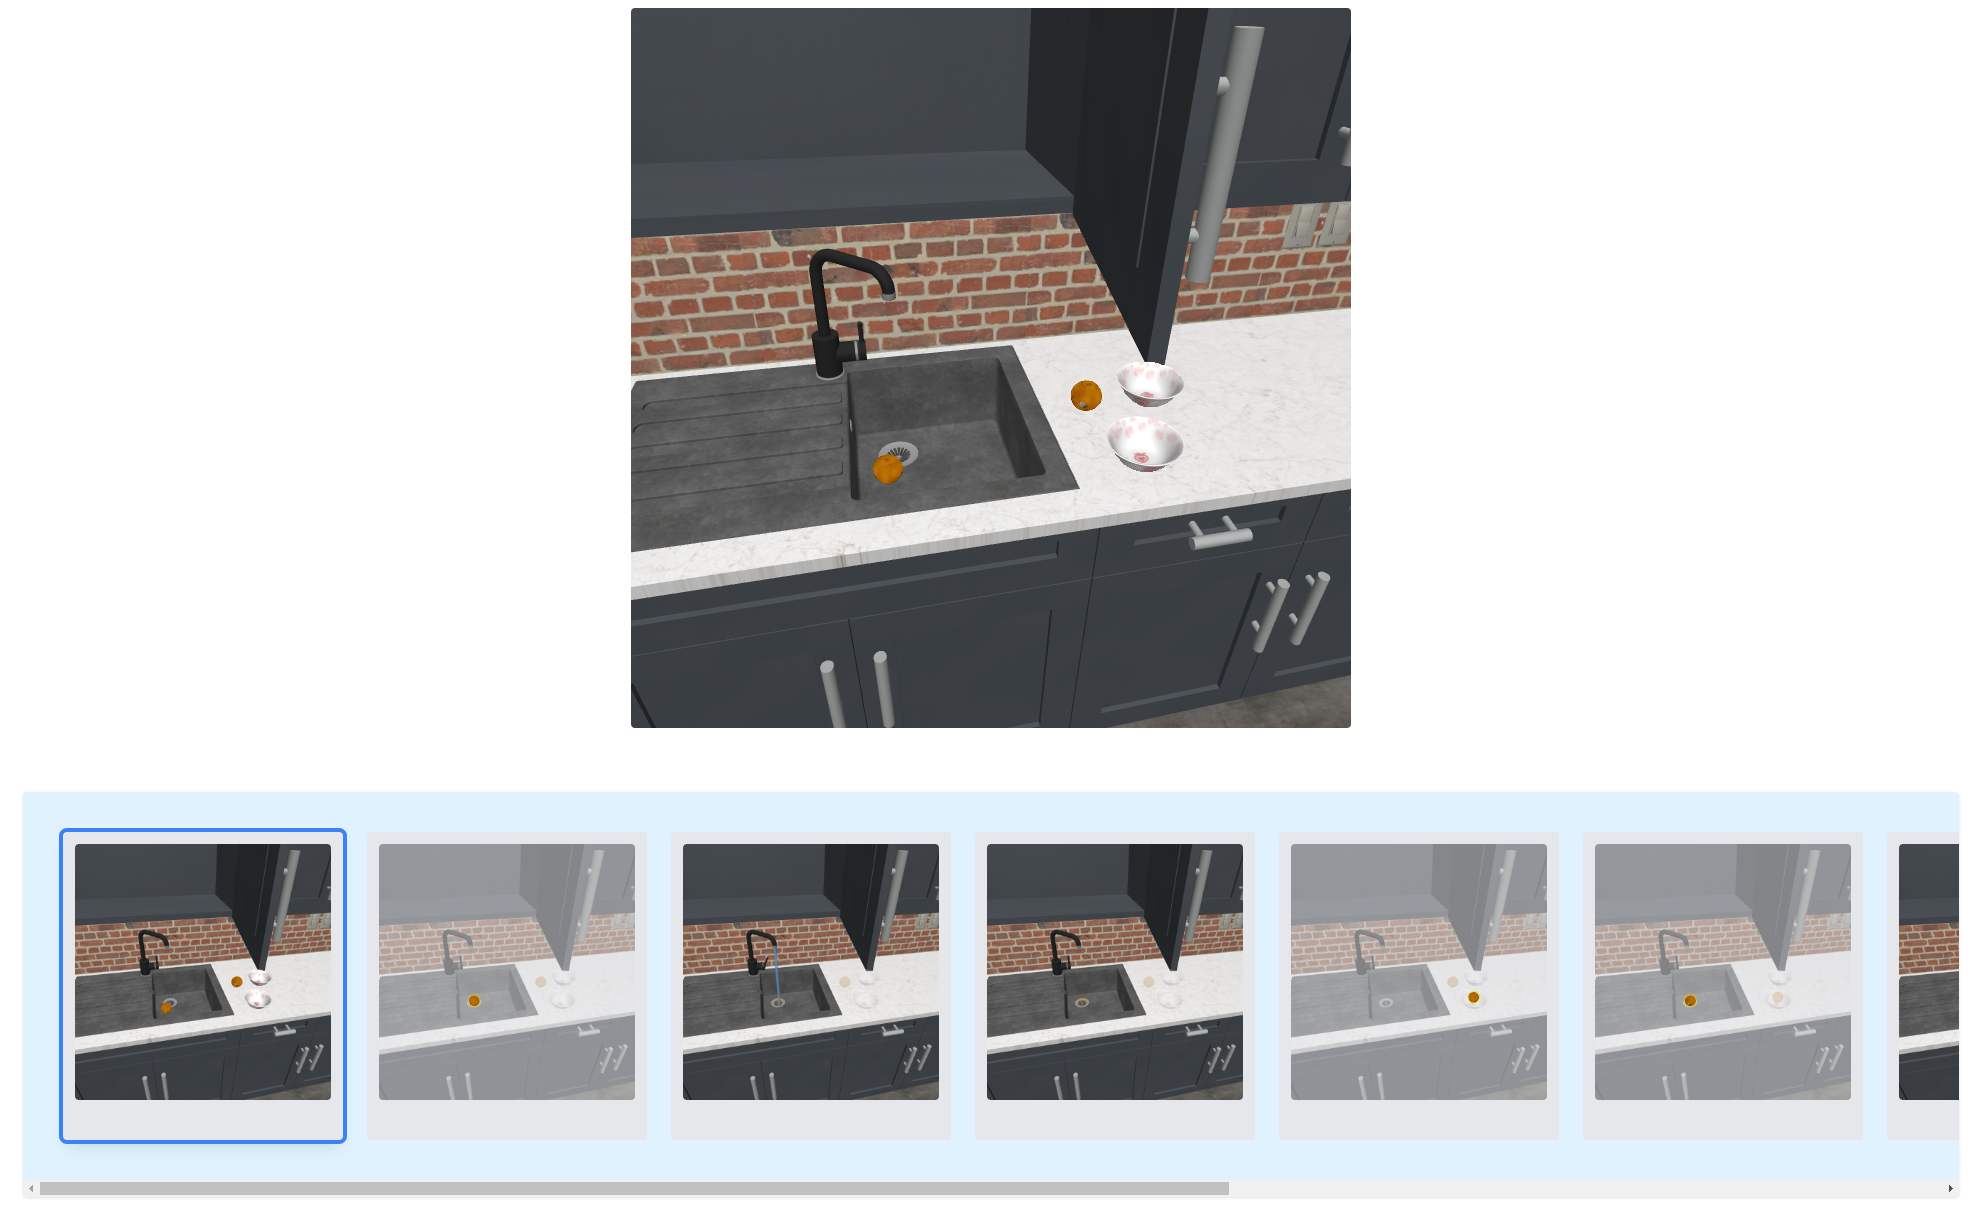
\includegraphics[width=0.8\textwidth]{figures/Interface.png}}
\caption{\projname's user interface, consisting of an editor (top) and a timeline (bottom). The editor allows users to manipulate objects and fixtures in the environment, while the timeline displays the current state of the environment and the desired changes.}
\label{fig:interface}
\end{figure*}

\section{Implementation}
\noindent \emph{High-level system design.} \projname consists of two major components: a back-end server that manages models to generate the image representations for manipulation and enables features such as automatic captioning, and a user interface for viewing and editing the images, enabling users to create robot instructions. The server is realized as a Flask application that enables two-way communication between the models and the interface. The models are hosted as TCP sockets on workstations within the local network and communicate with the Flask server to respond to requests from the interface. The user interface is built using ReactJS. Our implementation for the user study utilizes images from kitchen environments created using Robocasa~\cite{nasiriany2024robocasa}. 

%% Python (Flask) + ZMQ + ReactJS

\subsection{Representing the robot's environment} 
\projname creates an initial representation of the robot's environment by extracting information about the objects and fixtures present in them. 

\noindent \emph{Background image generation.} \projname assumes access to a predefined list of plausible objects and fixture states within the environment (e.g., a drawer being able to open or close) as well as the initial state of all fixtures. These assumptions are justified, as any robot entering a new environment would undergo an initialization phase to understand its surroundings. However, this knowledge can also be provided by the user or inferred by other models. Using this knowledge, \projname is able to enumerate all possible states of the environment. Each combination of states is then used to generate a background image that represents the environment in that state. For instance, in a kitchen environment consisting of a drawer and a cabinet, one combination of states could be the drawer being open and the cabinet being closed. Each of these images can be generated using a variety of methods. 

We experimented with fine-tuning language-conditioned diffusion models~\cite{brooks2023instructpix2pix, black2023zero} to generate images representing the appropriate state change but found the quality of the generated images to be inconsistent. Instead, for our prototype used in the user study, we utilized GPT-4o to generate code to modify the state of the fixtures inside the Robocasa environment. We envision that this could be plausible in the future given that many existing applications of robots assume the existence of digital twins~\cite{li2024evaluating}. At the end of this process, \projname creates a background image for all possible states, and sets the background image to the one that represents the current state.

\noindent \emph{Generating interactable objects and fixtures.} In order to enable the direct manipulation of images, \projname begins by detecting items from the previously known plausible list of items. In our physical robot implementation, the list of plausible items can be determined by prompting GPT-4o. Next, \projname generates bounding boxes for any detected items using an open vocabulary object detector, OWLv2~\cite{minderer2024scaling}. Then, information about the detected objects are passed to a segmentation model, Segment Anything (SAM~\cite{kirillov2023segment}), to generate manipulable masks. For the user study prototype, objects can be hidden when generating the background image so there is no white space and direct manipulation is possible at this stage. However, for the physical robot implementation, \projname performs an inpainting step to eliminate white spaces behind the objects before the user manipulates them~\cite{suvorov2022resolution}. For detected fixtures, \projname generates interactable regions by creating bounding boxes around the fixtures and enabling mouse clicks within these regions to activate state changes. 

\noindent \emph{Initializing the environment and state.} Upon generating backgrounds as well as representing objects and fixtures, the server transmits this information to the user interface. The environment describes static information about the environment, such as the background image and the interactable regions, while the state describes the current state of the environment. Once this information is received, the user interface renders the initial state of the environment as a step in the timeline represented as an SVG image.

\noindent \emph{Manipulating environment state.} The user can interact with the environment by manipulating objects and fixtures. Each time a new step is created, a new environment state is generated by copying the previous step and updating the data about any objects that moved or fixtures that changed state. When the user interacts with the interface, the system creates a new step by copying the representation of the previous step while updating data about any objects that moved. 

% After processing the initial state of all fixtures, the background image, generated masks, and bounding boxes for the fixtures are sent to user interface and rendered as a an SVG image inside a step. When the user clicks the initial step, the underlying representation is rendered inside an image editing application (\mk{CITE website}). The editor enables simple interactions such as the selection, deselection, and manipulating individual objects. When the user performs direct manipulations on one or more objects, the system creates a new step by copying the representation of the previous step while updating data about any objects that moved. To enable interactable fixtures, bounding boxes containing the location of fixtures are utilized to detect mouse clicks within this region, which activates a state change. When changing state, the current state variable is updated and the corresponding background image is retrieved and utilized when creating the step.

\noindent \emph{Predicting future steps (autocomplete)}

%Before the user begins providing instructions to the robot, \projname creates this initial representation to represent all objects and fixtures that are present in the environment, and determines the initial state. We assume access to the initial state of fixtures in the environment, such as the presence and number of cabinets, drawers, and sinks. For instance, a sample initial state could 


%This step can either be performed manually by a user when introducing their robot to their home, or automatically using models. 



% Describe how we make this by enumerating states 

% Sim/Susie/GPT

% How we make masks

% How we make interactable regions

\section{Evaluation}
We evaluated \projname through a controlled user study with twelve participants recruited using university and professional networks. Specifically, we compare an instance of \projname to a language-based method. The choice of a language-based method for comparison is based on its widespread deployment to instruct robots~\cite{team2024octo, zha2023distilling}.

\emph{Conditions.} To enable a fair comparison of each modality, we omitted all the language features of \projname, such as captioning and manipulating images using text (\mk: add feature names). Further, we also excluded all the intelligent features in \projname including autocomplete at the manipulation and step levels. For the language condition, we re-purposed \projname and replaced all image-based interactions with text. Instead of populating images in the timeline, the user populates the timeline with steps that consist of text. For the image-based method in \projname, we omit all language-based features (e.g., modifying images with captions) as well as autocomplete at the manipulation and step levels. In both the conditions, participants provided instructions pertaining to one object at a time, reflecting the current capabilities of robots, which typically handle single-object manipulation. Further, most language-conditioned robot policies, including foundation models, follow a similar approach, executing single language instructions at a time. While large language models can interpret more abstract instructions and decompose them, they are prone to errors and often require corrections~\cite{zha2023distilling}.

\emph{Study design.} The study utilizes a within-subjects design with two conditions--image and text--that are counterbalanced to minimize ordering effects (see Figure X for a full diagram). Within each condition, participants complete four tasks where they instruct a robot to complete kitchen manipulation tasks. The tasks include \textit{Organizing Pantry}, \textit{Sorting Fruits}, \textit{Preparing Stirfry}, and \textit{Washing Dishes}. Within each condition, the four tasks were randomly assigned. After both condition blocks, participants complete a freeform task to experiment with the features that were excluded from \projname. Details of the individual tasks can be found in the appendices (\mk{link}) and the website.

% To complete these tasks, the participant is provided the initial robot state as an image and a desired goal image. 

%%%% STATS about them like age, gender, etc. 

\emph{Measures.} In the study, we collected data about participants' performance when using both methods. Quantitative measures include task completion time and number of errors, which were determined by comparison to an \textit{oracle} representation of the task established a priori by two researchers. We also measured subjective perceptions of the interfaces, including participants' confidence in correctly communicating their intent to the robot, workload (NASA TLX~\cite{hart2006nasa}), and usability (SUS~\cite{bangor2008empirical}).

\emph{Procedure.} Participants first provided consent and completed a pre-study questionnaire assessing their familiarity with robots and instructing them. After watching a video tutorial introducing \projname and the text-based method and brief experimentation with both interfaces, participants began one of the two study condition blocks. Between tasks, participants rated how confident they were that the robot could understand their instructions unambiguously. At the end of each condition block, two questionnaires (NASA TLX and SUS) were administered to assess workload and usability, respectively. At the end of the study, participants rated their preference for the text-based interface compared to the image-based interface. Lastly, we conducted a brief interview probing participants about various aspects of both interfaces.







\section{Discussion}
\section{Conclusion}
\section*{Appendix}

% \subsection{Figures and Tables}
% \paragraph{Positioning Figures and Tables} Place figures and tables at the top and 
% bottom of columns. Avoid placing them in the middle of columns. Large 
% figures and tables may span across both columns. Figure captions should be 
% below the figures; table heads should appear above the tables. Insert 
% figures and tables after they are cited in the text. Use the abbreviation 
% ``Fig.~\ref{fig}'', even at the beginning of a sentence.

% \begin{table}[htbp]
% \caption{Table Type Styles}
% \begin{center}
% \begin{tabular}{|c|c|c|c|}
% \hline
% \textbf{Table}&\multicolumn{3}{|c|}{\textbf{Table Column Head}} \\
% \cline{2-4} 
% \textbf{Head} & \textbf{\textit{Table column subhead}}& \textbf{\textit{Subhead}}& \textbf{\textit{Subhead}} \\
% \hline
% copy& More table copy$^{\mathrm{a}}$& &  \\
% \hline
% \multicolumn{4}{l}{$^{\mathrm{a}}$Sample of a Table footnote.}
% \end{tabular}
% \label{tab1}
% \end{center}
% \end{table}

% \begin{figure}[htbp]
% \centerline{\includegraphics{fig1.png}}
% \caption{Example of a figure caption.}
% \label{fig}
% \end{figure}

% Figure Labels: Use 8 point Times New Roman for Figure labels. Use words 
% rather than symbols or abbreviations when writing Figure axis labels to 
% avoid confusing the reader. As an example, write the quantity 
% ``Magnetization'', or ``Magnetization, M'', not just ``M''. If including 
% units in the label, present them within parentheses. Do not label axes only 
% with units. In the example, write ``Magnetization (A/m)'' or ``Magnetization 
% \{A[m(1)]\}'', not just ``A/m''. Do not label axes with a ratio of 
% quantities and units. For example, write ``Temperature (K)'', not 
% ``Temperature/K''.

% \section*{Acknowledgment}

% The preferred spelling of the word ``acknowledgment'' in America is without 
% an ``e'' after the ``g''. Avoid the stilted expression ``one of us (R. B. 
% G.) thanks $\ldots$''. Instead, try ``R. B. G. thanks$\ldots$''. Put sponsor 
% acknowledgments in the unnumbered footnote on the first page.

% \section*{References}

% Please number citations consecutively within brackets \cite{b1}. The 
% sentence punctuation follows the bracket \cite{b2}. Refer simply to the reference 
% number, as in \cite{b3}---do not use ``Ref. \cite{b3}'' or ``reference \cite{b3}'' except at 
% the beginning of a sentence: ``Reference \cite{b3} was the first $\ldots$''

% Number footnotes separately in superscripts. Place the actual footnote at 
% the bottom of the column in which it was cited. Do not put footnotes in the 
% abstract or reference list. Use letters for table footnotes.

% Unless there are six authors or more give all authors' names; do not use 
% ``et al.''. Papers that have not been published, even if they have been 
% submitted for publication, should be cited as ``unpublished'' \cite{b4}. Papers 
% that have been accepted for publication should be cited as ``in press'' \cite{b5}. 
% Capitalize only the first word in a paper title, except for proper nouns and 
% element symbols.

% For papers published in translation journals, please give the English 
% citation first, followed by the original foreign-language citation \cite{b6}.

% \begin{thebibliography}{00}
% \bibitem{b1} G. Eason, B. Noble, and I. N. Sneddon, ``On certain integrals of Lipschitz-Hankel type involving products of Bessel functions,'' Phil. Trans. Roy. Soc. London, vol. A247, pp. 529--551, April 1955.
% \bibitem{b2} J. Clerk Maxwell, A Treatise on Electricity and Magnetism, 3rd ed., vol. 2. Oxford: Clarendon, 1892, pp.68--73.
% \bibitem{b3} I. S. Jacobs and C. P. Bean, ``Fine particles, thin films and exchange anisotropy,'' in Magnetism, vol. III, G. T. Rado and H. Suhl, Eds. New York: Academic, 1963, pp. 271--350.
% \bibitem{b4} K. Elissa, ``Title of paper if known,'' unpublished.
% \bibitem{b5} R. Nicole, ``Title of paper with only first word capitalized,'' J. Name Stand. Abbrev., in press.
% \bibitem{b6} Y. Yorozu, M. Hirano, K. Oka, and Y. Tagawa, ``Electron spectroscopy studies on magneto-optical media and plastic substrate interface,'' IEEE Transl. J. Magn. Japan, vol. 2, pp. 740--741, August 1987 [Digests 9th Annual Conf. Magnetics Japan, p. 301, 1982].
% \bibitem{b7} M. Young, The Technical Writer's Handbook. Mill Valley, CA: University Science, 1989.
% \end{thebibliography}
% \vspace{12pt}
% \color{red}
% IEEE conference templates contain guidance text for composing and formatting conference papers. Please ensure that all template text is removed from your conference paper prior to submission to the conference. Failure to remove the template text from your paper may result in your paper not being published.

\bibliographystyle{IEEEtran}
\bibliography{references}

\end{document}
